\documentclass[11pt, a4paper]{article}

\usepackage[margin=1in]{geometry}
\usepackage[utf8]{inputenc}
\usepackage[french]{babel}
\usepackage{hyperref}
\usepackage{ebgaramond}
\usepackage{pdfpages}

\hypersetup{
    colorlinks=true,
    linkcolor=black,
    urlcolor=blue,
    citecolor=black
}

\pagestyle{empty}
\parindent=0pt
\parskip=12pt

\begin{document}

% Title Page
{\centering\Large\textbf{Publications Pertinentes}\par
\textbf{Contribution Récentes en Gouvernance et Gestion de l'Intelligence Artificielle}\par}

\vspace{24pt}

\textbf{Carlos Denner dos Santos}

Candidature — Poste de Professeure ou Professeur en Gestion de l'Intelligence Artificielle

Université de Sherbrooke, Département SIMQG

\vspace{12pt}

{\textit{Novembre 2025}}

\vspace{24pt}

\hrule

\vspace{24pt}

\section*{Publications Incluses}

\begin{enumerate}
    \item \textbf{Almeida, P. G. R. \& Santos, C. D.} (2025). \textit{Artificial Intelligence Governance: Understanding How Public Organizations Implement IT}. \textbf{Government Information Quarterly}, 42(1), 102003.
    
    \textit{Impact and Relevance:} Publication la plus récente (2025). Étude empirique de la mise en œuvre de la gouvernance de l'IA dans 28 organisations publiques sur cinq continents. Directement alignée avec l'axe 1 du programme de recherche proposé.
    
    \item \textbf{Almeida, P. G. R., Santos, C. D., \& Farias, J. S.} (2021). \textit{Artificial Intelligence Regulation: A Framework for Governance}. \textbf{Ethics and Information Technology}, 23(3), 505--525.
    
    \textit{Impact and Relevance:} Publication fondatrice du programme de gouvernance de l'IA. Propose un cadre intégrateur pour la régulation de l'IA. Cite plus de 200 fois. Établit les concepts fondamentaux qui structurent le programme de recherche proposé à Sherbrooke.
    
    \item \textbf{Moura, P. J., Santos, C. D., Bellini, C. G. P., \& Dias, J. J. L.} (2024). \textit{The Over-Concentration of Innovation and Firm-Specific Knowledge in the Artificial Intelligence Industry}. \textbf{Journal of the Knowledge Economy}, 15(4), 20547--20577.
    
    \textit{Impact and Relevance:} Publication 2024 portant directement sur l'industrie de l'IA. Analyse la concentration de l'innovation et des connaissances spécifiques aux entreprises — enjeu clé de la durabilité et de l'impact des systèmes d'IA dans les organisations (Axe 3 du programme de recherche).

\end{enumerate}

\vspace{24pt}

\textbf{Note:} Les trois publications ci-après sont présentées dans l'ordre de leur pertinence pour le poste. Elles couvrent collectivement : (1) la recherche empirique récente sur la gouvernance de l'IA dans les organisations, (2) le cadre conceptuel fondateur en régulation de l'IA, et (3) une preuve antérieure de rigueur en gouvernance organisationnelle complexe.

\newpage

% Include PDF 1: GIQ 2025
\includepdf[pages=-]{Publications/1-s2.0-S0740624X24000959-main.pdf}

\newpage

% Include PDF 2: Ethics & IT 2021
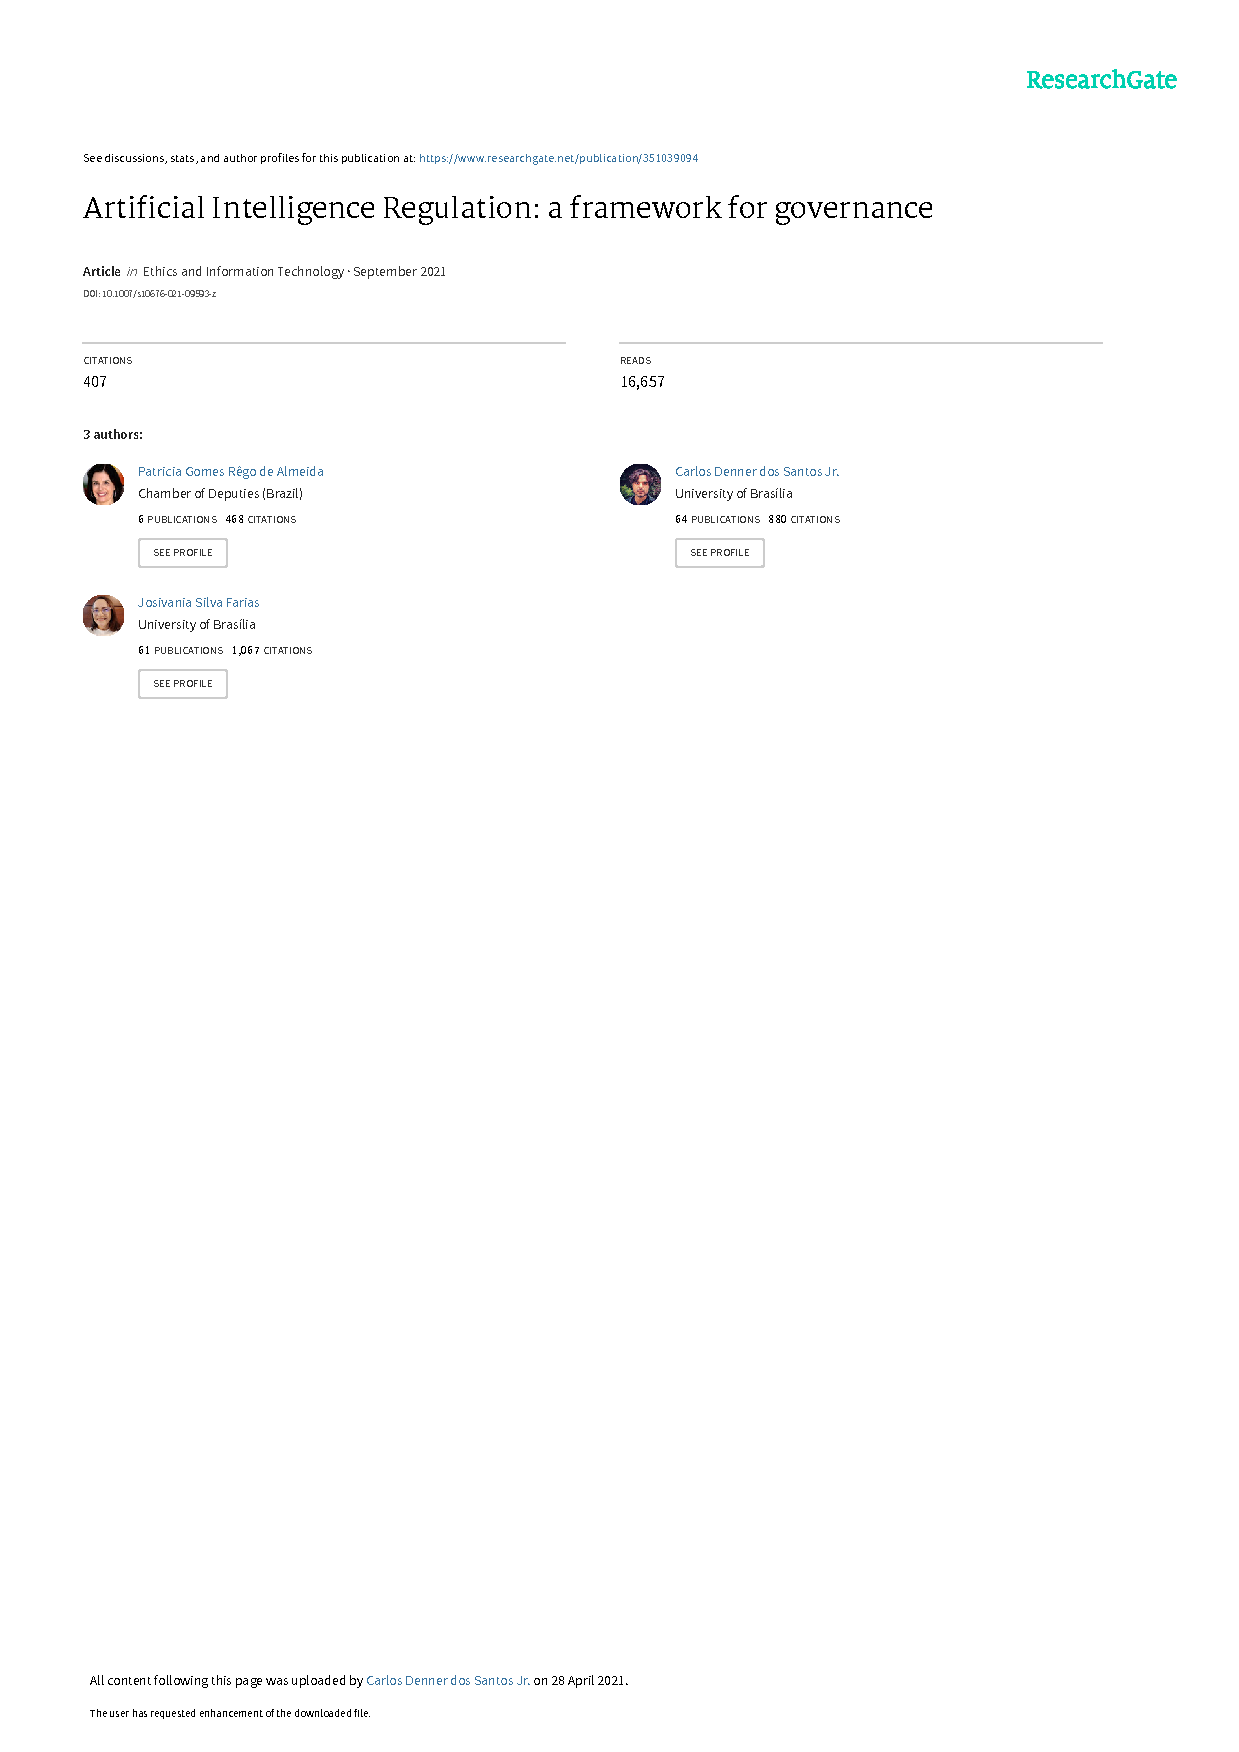
\includepdf[pages=-]{Publications/Almeida2021_Article_ArtificialIntelligenceRegulati.pdf}

\newpage

% Include PDF 3: Knowledge Economy 2024
\includepdf[pages=-]{Publications/The_Over-Concentration_of_Innovation_and_Firm-Spec.pdf}

\end{document}
